\documentclass[11pt]{article}

\usepackage[utf8]{inputenc}
\usepackage[spanish]{babel}
\usepackage{amsmath}
\usepackage{a4wide}
\usepackage{graphicx}
\usepackage{minted}

\title{Métodos Numéricos II - Cuerda vibrante}
\author{Unai Aguilera Irazabal\\ DNI: 45663055M}

\begin{document}
\maketitle
\tableofcontents

\pagebreak
\renewcommand{\tablename}{Tabla}

\section{Introducción}
La ecuación que define el movimiento de una cuerda vibrante amortiguada es la siguiente

\begin{equation}
\frac{\partial^2 y}{\partial{t^2}} = \frac{Tg}{\rho}\frac{\partial^2 y}{\partial{x^2}} 
	- B\frac{\partial y}{\partial{t}}
\label{eq:cuerda}
\end{equation}

donde $B=2.0$ es la magnitud de la fuerza de amortiguamiento, $T=10$ Kg su tensión,
$\rho = 500$ g/m su densidad lineal y $g = 9.8$ m/s la aceleración de la gravedad. 

La ecuación de la cuerda vibrante es una ecuación de tipo hiperbólico que para poder ser
resuelta es necesario conocer los valores de frontera (posición y/o velocidad de los extremos) y
dos condiciones iniciales, los valores de la posición y la velocidad de cada punto en el instante
inicial $t=0$.
En el caso del problema propuesto, las condiciones iniciales son

\begin{subequations}
\begin{flalign}
	&y(x)|_{t=0} = \frac{x}{3},~~~~~~~~~~~~~~~~~~ 0 <= x < \frac{3}{5}\\
	&y(x)|_{t=0} = \frac{1}{2}(1 - x),~~~~~~~~~ \frac{3}{5} <= x <= 1\\
	&\frac{\partial{y}}{\partial{t}}|_{t=0} = x(x-1)
\end{flalign}
\label{eq:condiciones_iniciales}
\end{subequations}

donde $y(x)|_{t=0}$ determina la posición inicial de la cuerda y se trata de una función
por partes pero continúa.

\section{Método de resolución}
La ecuación \eqref{eq:cuerda} puede ser resuelta de forma numérica mediante la substitución
de las derivadas por aproximaciones con diferencias finitas. En este caso, se utilizan las
siguientes aproximaciones para cada una de las derivadas, siendo las dos primeras
diferencias de tipo central y la última de tipo posterior o adelantada.

\begin{subequations}
\begin{flalign}
	&\frac{\partial^2 y}{\partial{x^2}} = \frac{y^j_{i+1} - 2y^j_i + y^j_{i-1}}{(\Delta{x})^2}\\
	&\frac{\partial^2 y}{\partial{t^2}} = \frac{y^{j+1}_i - 2y^j_i + y^{j-1}_i}{(\Delta{t})^2}\\
	&\frac{\partial{y}}{\partial{t}} = \frac{y^{j+1}_i - y^{j-1}_i}{2\Delta{t}}
\end{flalign}
\end{subequations}

Substituyendo las aproximaciones en la ecuación \eqref{eq:cuerda}, se obtiene la siguiente
expresión

\begin{equation}
\frac{y^{j+1}_i - 2y^j_i + y^{j-1}_i}{(\Delta{t})^2} = 
	\frac{Tg}{\rho}\frac{y^j_{i+1} - 2y^j_i + y^j_{i-1}}{(\Delta{x})^2}
	- B \frac{y^{j+1}_i - y^{j-1}_i}{2\Delta{t}}
\end{equation}

en donde reordenando términos 

\begin{equation}
y^{j+1}_{i} - 2y^{j}_i + y^{j-1}_i = \frac{Tg(\Delta{t})^2}{\rho(\Delta{x})^2}
	(y^j_{i+1} - 2y^j_i + y^j_{i-1}) - \frac{B\Delta{t}}{2}(y^{j+1}_i - y^{j-1}_i)
\label{eq:aproximacion}
\end{equation}

Si en la expresión anterior el valor $\frac{Tg(\Delta{t})^2}{\rho(\Delta{x})^2}$ se iguala
a la unidad, valor máximo que permite estabilidad, y se despeja el desplazamiento $y^{j+1}_i$,
se obtiene la siguiente expresión

\begin{equation}
y^{j+1}_i = \frac{y^j_{i+1} + y^j_{i-1} + (\frac{B\Delta{t}}{2} - 1)y^{j-1}_i}{(\frac{B\Delta{t}}{2} + 1)}
\label{eq:pasos_siguientes}
\end{equation}

que permite calcular el valor de un nodo i en un paso de tiempo posterior a partir de la
información de los nodos vecinos a derecha e izquierda y del valor del propio nodo en un
instante anterior.

A partir de la simplificación realizada anteriormente puede obtenerse que 

\begin{equation}
\Delta{t} = \frac{\Delta{x}}{\sqrt{\frac{Tg}{\rho}}}
\label{eq:paso_tiempo}
\end{equation}

lo que permite determinar el tamaño del paso de tiempo $\Delta{t}$ adecuado a partir de las
características físicas de la cuerda vibrante y del paso espacial $\Delta{x}$ definido para
la subdivisión de la cuerda en intervalos de diferencias finitas durante la aproximación de
las derivadas.

La expresión \eqref{eq:pasos_siguientes} permite obtener la evolución del sistema
en todo paso de tiempo salvo en el primero ($0 \rightarrow 1$), ya que hace referencia a
un instante anterior al inicio $y^{-1}$. Sin embargo, esta información puede determinarse a
partir del conocimiento de la velocidad inicial del sistema proporcionada por
$\frac{\partial{y}}{\partial{x}}|_{t=0}$ en las condiciones iniciales.
Así, en el paso inicial

\begin{equation}
\frac{y^1_i - y^{-1}_i}{2\Delta{t}} = \frac{\partial{y}}{\partial{x}}|_{t=0}
\label{eq:aprox_derivada}
\end{equation}

y a partir de la ecuación \eqref{eq:aproximacion} y substituyendo nuevamente el valor de 
$\frac{Tg(\Delta{t})^2}{\rho(\Delta{x})^2}$ por la unidad se obtiene

\begin{equation}
y^{j+1}_i = y^{j}_{i+1} + y^{j}_{j-1} - y^{j-1}_i - \frac{B\Delta{t}}{2}(y^{j+1}_i - y^{j-1}_i)
\end{equation}

donde para $j=0$ y substituyendo la aproximación dada por la ecuación
\eqref{eq:aprox_derivada} y, tras despejar nuevamente $y^{j+1}_i$, se obtiene la siguiente
expresión para el paso inicial del método numérico

\begin{equation}
y^1_i = \frac{y^0_{i+1} + y^0_{i-1}}{2} + \Delta{t}\frac{\partial{y}}{\partial{x}}|_{t=0}
	- \frac{B\Delta{t}^2}{2}\frac{\partial{y}}{\partial{x}}|_{t=0}
\label{eq:paso_inicial}
\end{equation}

\section{Caso no amortiguado}
Para el caso de la cuerda vibrante sin amortiguamiento, las ecuaciones para su resolución
mediante el método numérico por aproximación de diferencias finitas se obtienen haciendo
$B=0$ en las ecuaciones \eqref{eq:pasos_siguientes} y \eqref{eq:paso_inicial}. Siendo
necesario además llevar a cabo la substitución de $\frac{\partial{y}}{\partial{x}}|_{t=0}$
por la expresión indicada en las condiciones iniciales del problema dadas en
\eqref{eq:condiciones_iniciales}.

\begin{subequations}
\begin{flalign}
	&y^1_i = \frac{y^0_{i+1} + y^0_{i-1}}{2} + x(x-1)\Delta{t}\\
	&y^{j+1}_i = y^j_{i+1} + y^j_{i-1} - y^{j-1}_i
\end{flalign}
\end{subequations}

Utilizando el esquema anterior de forma iterativa e inicializando las posiciones de
los nodos de la cuerda para $t=0$ según las condiciones indicadas en el problema
\eqref{eq:condiciones_iniciales} se obtienen los resultados recogidos en la Tabla 
\ref{tab:est_freq}. Esta muestra la posición de la cuerda en pasos consecutivos de tiempo 
utilizando un espaciado de $\Delta{x} = 0.1$ cm para la subdivisión de la misma.

En la Tabla \ref{tab:est_freq} se observa que la cuerda vuelve a su estado inicial cuando
han transcurrido 20 pasos de tiempo. Así, utilizando la ecuación \eqref{eq:paso_tiempo},
de donde es posible obtener el valor de un paso de tiempo, se calcula que
$\Delta{t} = 0.0071$ s mediante la substitución de los parámetros de la cuerda y el
intervalo espacial elegido. Finalmente, a partir del tamaño de un paso de tiempo se
obtiene que

\begin{equation}
f = \frac{1}{n \Delta{t}} = \frac{1}{20 * 0.0071} = 7.04~Hz
\end{equation}

\begin{table}
\center
\begin{small}
\begin{tabular}{ c c c c c c c c c c c c }
\hline
Paso & 0.00 & 0.10 & 0.20 & 0.30 & 0.40 & 0.50 & 0.60 & 0.70 & 0.80 & 0.90 & 1.00 \\
\hline
\hline
0 & 0.00 & 0.03 & 0.07 & 0.10 & 0.13 & 0.17 & 0.20 & 0.15 & 0.10 & 0.05 & 0.00 \\
1 & 0.00 & 0.03 & 0.07 & 0.10 & 0.13 & 0.16 & 0.16 & 0.15 & 0.10 & 0.05 & 0.00 \\
2 & 0.00 & 0.03 & 0.06 & 0.10 & 0.13 & 0.12 & 0.11 & 0.11 & 0.10 & 0.05 & 0.00 \\
3 & 0.00 & 0.03 & 0.06 & 0.10 & 0.09 & 0.08 & 0.07 & 0.06 & 0.06 & 0.05 & 0.00 \\
4 & 0.00 & 0.03 & 0.06 & 0.05 & 0.04 & 0.04 & 0.03 & 0.02 & 0.01 & 0.01 & 0.00 \\
5 & 0.00 & 0.03 & 0.02 & 0.01 & 0.00 & -0.01 & -0.01 & -0.02 & -0.03 & -0.04 & 0.00 \\
6 & 0.00 & -0.01 & -0.02 & -0.03 & -0.04 & -0.05 & -0.06 & -0.06 & -0.07 & -0.04 & 0.00 \\
7 & 0.00 & -0.05 & -0.06 & -0.07 & -0.08 & -0.09 & -0.10 & -0.10 & -0.07 & -0.03 & 0.00 \\
8 & 0.00 & -0.05 & -0.10 & -0.11 & -0.12 & -0.13 & -0.14 & -0.10 & -0.07 & -0.03 & 0.00 \\
9 & 0.00 & -0.05 & -0.10 & -0.15 & -0.16 & -0.17 & -0.14 & -0.10 & -0.07 & -0.03 & 0.00 \\
10 & 0.00 & -0.05 & -0.10 & -0.15 & -0.20 & -0.17 & -0.13 & -0.10 & -0.07 & -0.03 & 0.00 \\
11 & 0.00 & -0.05 & -0.10 & -0.15 & -0.16 & -0.16 & -0.13 & -0.10 & -0.07 & -0.03 & 0.00 \\
12 & 0.00 & -0.05 & -0.10 & -0.11 & -0.11 & -0.12 & -0.13 & -0.10 & -0.06 & -0.03 & 0.00 \\
13 & 0.00 & -0.05 & -0.06 & -0.06 & -0.07 & -0.08 & -0.09 & -0.10 & -0.06 & -0.03 & 0.00 \\
14 & 0.00 & -0.01 & -0.01 & -0.02 & -0.03 & -0.04 & -0.04 & -0.05 & -0.06 & -0.03 & 0.00 \\
15 & 0.00 & 0.04 & 0.03 & 0.02 & 0.01 & 0.01 & -0.00 & -0.01 & -0.02 & -0.03 & 0.00 \\
16 & 0.00 & 0.04 & 0.07 & 0.06 & 0.06 & 0.05 & 0.04 & 0.03 & 0.02 & 0.01 & 0.00 \\
17 & 0.00 & 0.03 & 0.07 & 0.10 & 0.10 & 0.09 & 0.08 & 0.07 & 0.06 & 0.05 & 0.00 \\
18 & 0.00 & 0.03 & 0.07 & 0.10 & 0.14 & 0.13 & 0.12 & 0.11 & 0.10 & 0.05 & 0.00 \\
19 & 0.00 & 0.03 & 0.07 & 0.10 & 0.14 & 0.17 & 0.16 & 0.15 & 0.10 & 0.05 & 0.00 \\
\hline
20 & 0.00 & 0.03 & 0.07 & 0.10 & 0.13 & 0.17 & 0.20 & 0.15 & 0.10 & 0.05 & 0.00 \\
\hline
21 & 0.00 & 0.03 & 0.07 & 0.10 & 0.13 & 0.16 & 0.16 & 0.15 & 0.10 & 0.05 & 0.00 \\
% 22 & 0.00 & 0.03 & 0.06 & 0.10 & 0.13 & 0.12 & 0.11 & 0.11 & 0.10 & 0.05 & 0.00 \\
% 23 & 0.00 & 0.03 & 0.06 & 0.10 & 0.09 & 0.08 & 0.07 & 0.06 & 0.06 & 0.05 & 0.00 \\
% 24 & 0.00 & 0.03 & 0.06 & 0.05 & 0.04 & 0.04 & 0.03 & 0.02 & 0.01 & 0.01 & 0.00 \\
% 25 & 0.00 & 0.03 & 0.02 & 0.01 & 0.00 & -0.01 & -0.01 & -0.02 & -0.03 & -0.04 & 0.00 \\
\end{tabular}
\end{small}
\caption{Resultados de la cuerda en vibración para $\Delta{x} = 0.1$ cm}
\label{tab:est_freq}
\end{table}

En la Tabla \ref{tab:est_velocidad} se recogen nuevamente los resultados para algunos nodos
usando el mismo intervalo espacial $\Delta{x} = 0.1$ cm. Sin embargo, en este caso se han
añadido también las velocidades de los puntos de la cuerda. Las velocidades han sido
calculadas utilizando las diferencias de posición entre dos instantes consecutivos de
tiempo de acuerdo al siguiente esquema de diferencias adelantado

\begin{equation}
\frac{\partial{y}}{\partial{t}} = \frac{y^{j + 1}_i - y^{j}_i}{\Delta{t}}
\end{equation} 

Puede observarse de nuevo que la velocidad inicial es recuperada en el paso de tiempo 20,
punto en el cual comienza a repetirse el ciclo de movimiento de la cuerda debido a que no
hay pérdida de energía por amortiguamiento.

\begin{table}[t]
\center
\begin{small}
\begin{tabular}{ c c c c c }
\hline
Paso & 0.30 & 0.40 & 0.50 & 0.60 \\
\hline
\hline
0 & 0.10 (-0.21) & 0.13 (-0.24) & 0.17 (-0.25) & 0.20 (-6.07) \\
1 & 0.10 (-0.19) & 0.13 (-0.22) & 0.16 (-6.06) & 0.16 (-6.05) \\
2 & 0.10 (-0.15) & 0.13 (-6.01) & 0.12 (-6.02) & 0.11 (-6.01) \\
3 & 0.10 (-5.92) & 0.09 (-5.95) & 0.08 (-5.96) & 0.07 (-5.95) \\
4 & 0.05 (-5.86) & 0.04 (-5.87) & 0.04 (-5.88) & 0.03 (-5.87) \\
5 & 0.01 (-5.80) & 0.00 (-5.79) & -0.01 (-5.78) & -0.01 (-5.79) \\
6 & -0.03 (-5.74) & -0.04 (-5.71) & -0.05 (-5.70) & -0.06 (-5.71) \\
7 & -0.07 (-5.68) & -0.08 (-5.65) & -0.09 (-5.64) & -0.10 (-5.65) \\
8 & -0.11 (-5.64) & -0.12 (-5.61) & -0.13 (-5.60) & -0.14 (0.22) \\
9 & -0.15 (0.21) & -0.16 (-5.59) & -0.17 (0.25) & -0.14 (0.24) \\
10 & -0.15 (0.21) & -0.20 (6.07) & -0.17 (0.25) & -0.13 (0.24) \\
11 & -0.15 (6.02) & -0.16 (6.05) & -0.16 (6.06) & -0.13 (0.22) \\
12 & -0.11 (5.98) & -0.11 (6.01) & -0.12 (6.02) & -0.13 (6.01) \\
13 & -0.06 (5.92) & -0.07 (5.95) & -0.08 (5.96) & -0.09 (5.95) \\
14 & -0.02 (5.86) & -0.03 (5.87) & -0.04 (5.88) & -0.04 (5.87) \\
15 & 0.02 (5.80) & 0.01 (5.79) & 0.01 (5.78) & -0.00 (5.79) \\
16 & 0.06 (5.74) & 0.06 (5.71) & 0.05 (5.70) & 0.04 (5.71) \\
17 & 0.10 (-0.15) & 0.10 (5.65) & 0.09 (5.64) & 0.08 (5.65) \\
18 & 0.10 (-0.19) & 0.14 (-0.22) & 0.13 (5.60) & 0.12 (5.61) \\
19 & 0.10 (-0.21) & 0.14 (-0.24) & 0.17 (-0.25) & 0.16 (5.59) \\
\hline
20 & 0.10 (-0.21) & 0.13 (-0.24) & 0.17 (-0.25) & 0.20 (-6.07) \\
\hline
21 & 0.10 (-0.19) & 0.13 (-0.22) & 0.16 (-6.06) & 0.16 (-6.05) \\
% 22 & 0.10 (-0.15) & 0.13 (-6.01) & 0.12 (-6.02) & 0.11 (-6.01) \\
% 23 & 0.10 (-5.92) & 0.09 (-5.95) & 0.08 (-5.96) & 0.07 (-5.95) \\
% 24 & 0.05 (-5.86) & 0.04 (-5.87) & 0.04 (-5.88) & 0.03 (-5.87) \\
\end{tabular}
\end{small}
\caption{Posición y velocidad de algunos nodos de la cuerda para $\Delta{x} = 0.1$ cm }
\label{tab:est_velocidad}
\end{table}

\subsection{Solución analítica}
\label{sec:sol_analitica}
La solución analítica en el caso de la cuerda vibrante puede obtenerse mediante el método
de separación de variables. Si en la ecuación \eqref{eq:cuerda} se realiza la siguiente
substitución

\begin{equation}
y(x,t) = u(x)v(t)
\end{equation}

es posible obtener el siguiente sistema de ecuaciones haciendo que cada parte de la ecuación
dependa únicamente de una variable e igualando cada lado a cierta constante $-K$.

\begin{subequations}
\begin{flalign}
	&\frac{v''(t)}{c^2v(t)} = -K\\
	&\frac{u''(x)}{u(x)} = -K
\end{flalign}
\label{eq:sistema_cuerda}
\end{subequations}

De acuerdo a las condiciones iniciales del problema sabemos que los extremos de la cuerda
están fijos en $u(0) = u(1) = 0$. Estas condiciones junto con segunda ecuación de las
anteriores

\begin{equation}
	u''(x) + Ku(x) = 0
\end{equation}

permiten plantear un problema de valores propios cuya solución viene dada por

\begin{equation}
	K = n^2\pi^2
\end{equation}

siendo las funciones propias correspondientes

\begin{equation}
	u_n(x) = c_n\sin{n\pi{x}}
\end{equation}

donde $c_n$ son constantes arbitrarias no nulas que deben ser determinadas.

A continuación se considera la otra ecuación de \eqref{eq:sistema_cuerda} con los
valores de K ya obtenidos

\begin{equation}
	v''(t) + c^2n^2\pi^2v(t) = 0
\end{equation}
 
La solución general para esta ecuación es para cada posible valor de $n$

\begin{equation}
	u_n(x) = c_{n,1}\cos{n\pi{c}t} + c_{n,2}\sin{n\pi{c}t}
\end{equation}

Al combinar los resultados anteriores en $y(x,t) = u(x)v(t)$ y absorber las constantes, se
obtiene que

\begin{equation}
	y_n(x,t) = (a_n\cos{n\pi{c}t} + b_n\sin{n\pi{c}t})\sin{n\pi{x}}
\end{equation}

Sin embargo, hay que tener en cuenta que la solución completa es la combinación lineal de
todos los posibles valores de n, por lo que finalmente

\begin{equation}
	y(x,t) = \sum\limits_{i=1}^\infty[a_n\cos{n\pi{c}t} + b_n\sin{n\pi{c}t}]\sin{n\pi{x}}
\label{eq:sol_analitica}
\end{equation}

Ahora ya pueden aplicarse las condiciones iniciales, que en el caso del problema son del
tipo

\begin{equation}
	y(x, 0) = f(x)~~~~~~~~~~~~~~\frac{\partial{y}}{\partial{t}}(x, 0) = g(x)
\end{equation}

obteniéndose de esta forma las siguientes condiciones que permiten determinar el valor de
las constantes $a_n$ y $b_n$

\begin{subequations}
\begin{flalign}
	&\sum\limits_{i=1}^\infty a_n \sin{n\pi{x}} = f(x)\\
	&\sum\limits_{i=1}^\infty b_n n\pi{c} \sin{n\pi{x}} = g(x)
\end{flalign}
\end{subequations}

Así, para obtener el valor de las $a_n$ es necesario resolver la serie de Fourier usando
la siguiente integral

\begin{equation}
	a_n = 2 \int_0^1 f(x) \sin{n\pi{x}}dx = 2[\int_0^\frac{3}{5} \frac{x}{3} \sin{n\pi{x}}dx
	+ \int_{\frac{3}{5}}^1 \frac{1}{2}(1-x) \sin{n\pi{x}}dx]
\end{equation}

obteniéndose mediante su solución la expresión analítica para cada $a_n$.

\begin{equation}
	a_n = 2 [\frac{\sin{n\pi{x}} - \pi{n}x\cos{n\pi{x}}}{3\pi^3n^3}\rvert_0^\frac{3}{5}
	+ [\frac{\sin(n\pi{x})}{2\pi^2n^2} + \frac{x\cos(n\pi{x})}{2\pi{n}} - \frac{\cos(n\pi{x})}{2\pi{n}}]\rvert_{\frac{3}{5}}^1]
\end{equation}

En el caso de $b_n$ se sigue el mismo procedimiento para resolver la integral

\begin{equation}
	b_n n\pi{c} = 2 \int_0^1 g(x) \sin{n\pi{x}}dx = 2 \int_0^1 x(x-1) \sin{n\pi{x}}dx 
\end{equation}

y obtener la siguiente expresión analítica

\begin{equation}
	b_n n\pi{c} = 2[\frac{(2 - \pi^2n^2(x-1)x)\cos{n\pi{x}} + \pi{n}(2x - 1)\sin{n\pi{x}}}{\pi^3n^3}]\rvert_0^1 
\end{equation}

Finalmente, a partir de las expresiones obtenidas para $a_n$ y $b_n$ es posible calcular
la posición de la cuerda para cada $y(x,t)$ utilizando la expresión analítica proporcionada
por la ecuación \eqref{eq:sol_analitica}.

El código Python que permite el cálculo de los valores analíticos para la posición de la
cuerda se muestra en la Figura \ref{fig:sol_analitica}. En todos los cálculos de la solución
analítica recogidos en este trabajo se han utilizado 100 elementos de la serie de Fourier,
tanto para $a_n$ como para $b_n$ con la finalidad de calcular la posición de la cuerda con
una precisión suficiente para considerarla como el caso exacto.

Una representación gráfica de la posición de la cuerda para diferentes pasos de tiempo
(0, 5, 10, 17) se muestra en la Figura \ref{fig:graficas}. En la figura se observan
diferentes posiciones de los nodos de la cuerda durante la realización de un ciclo de
vibración.

\begin{figure}
\centering
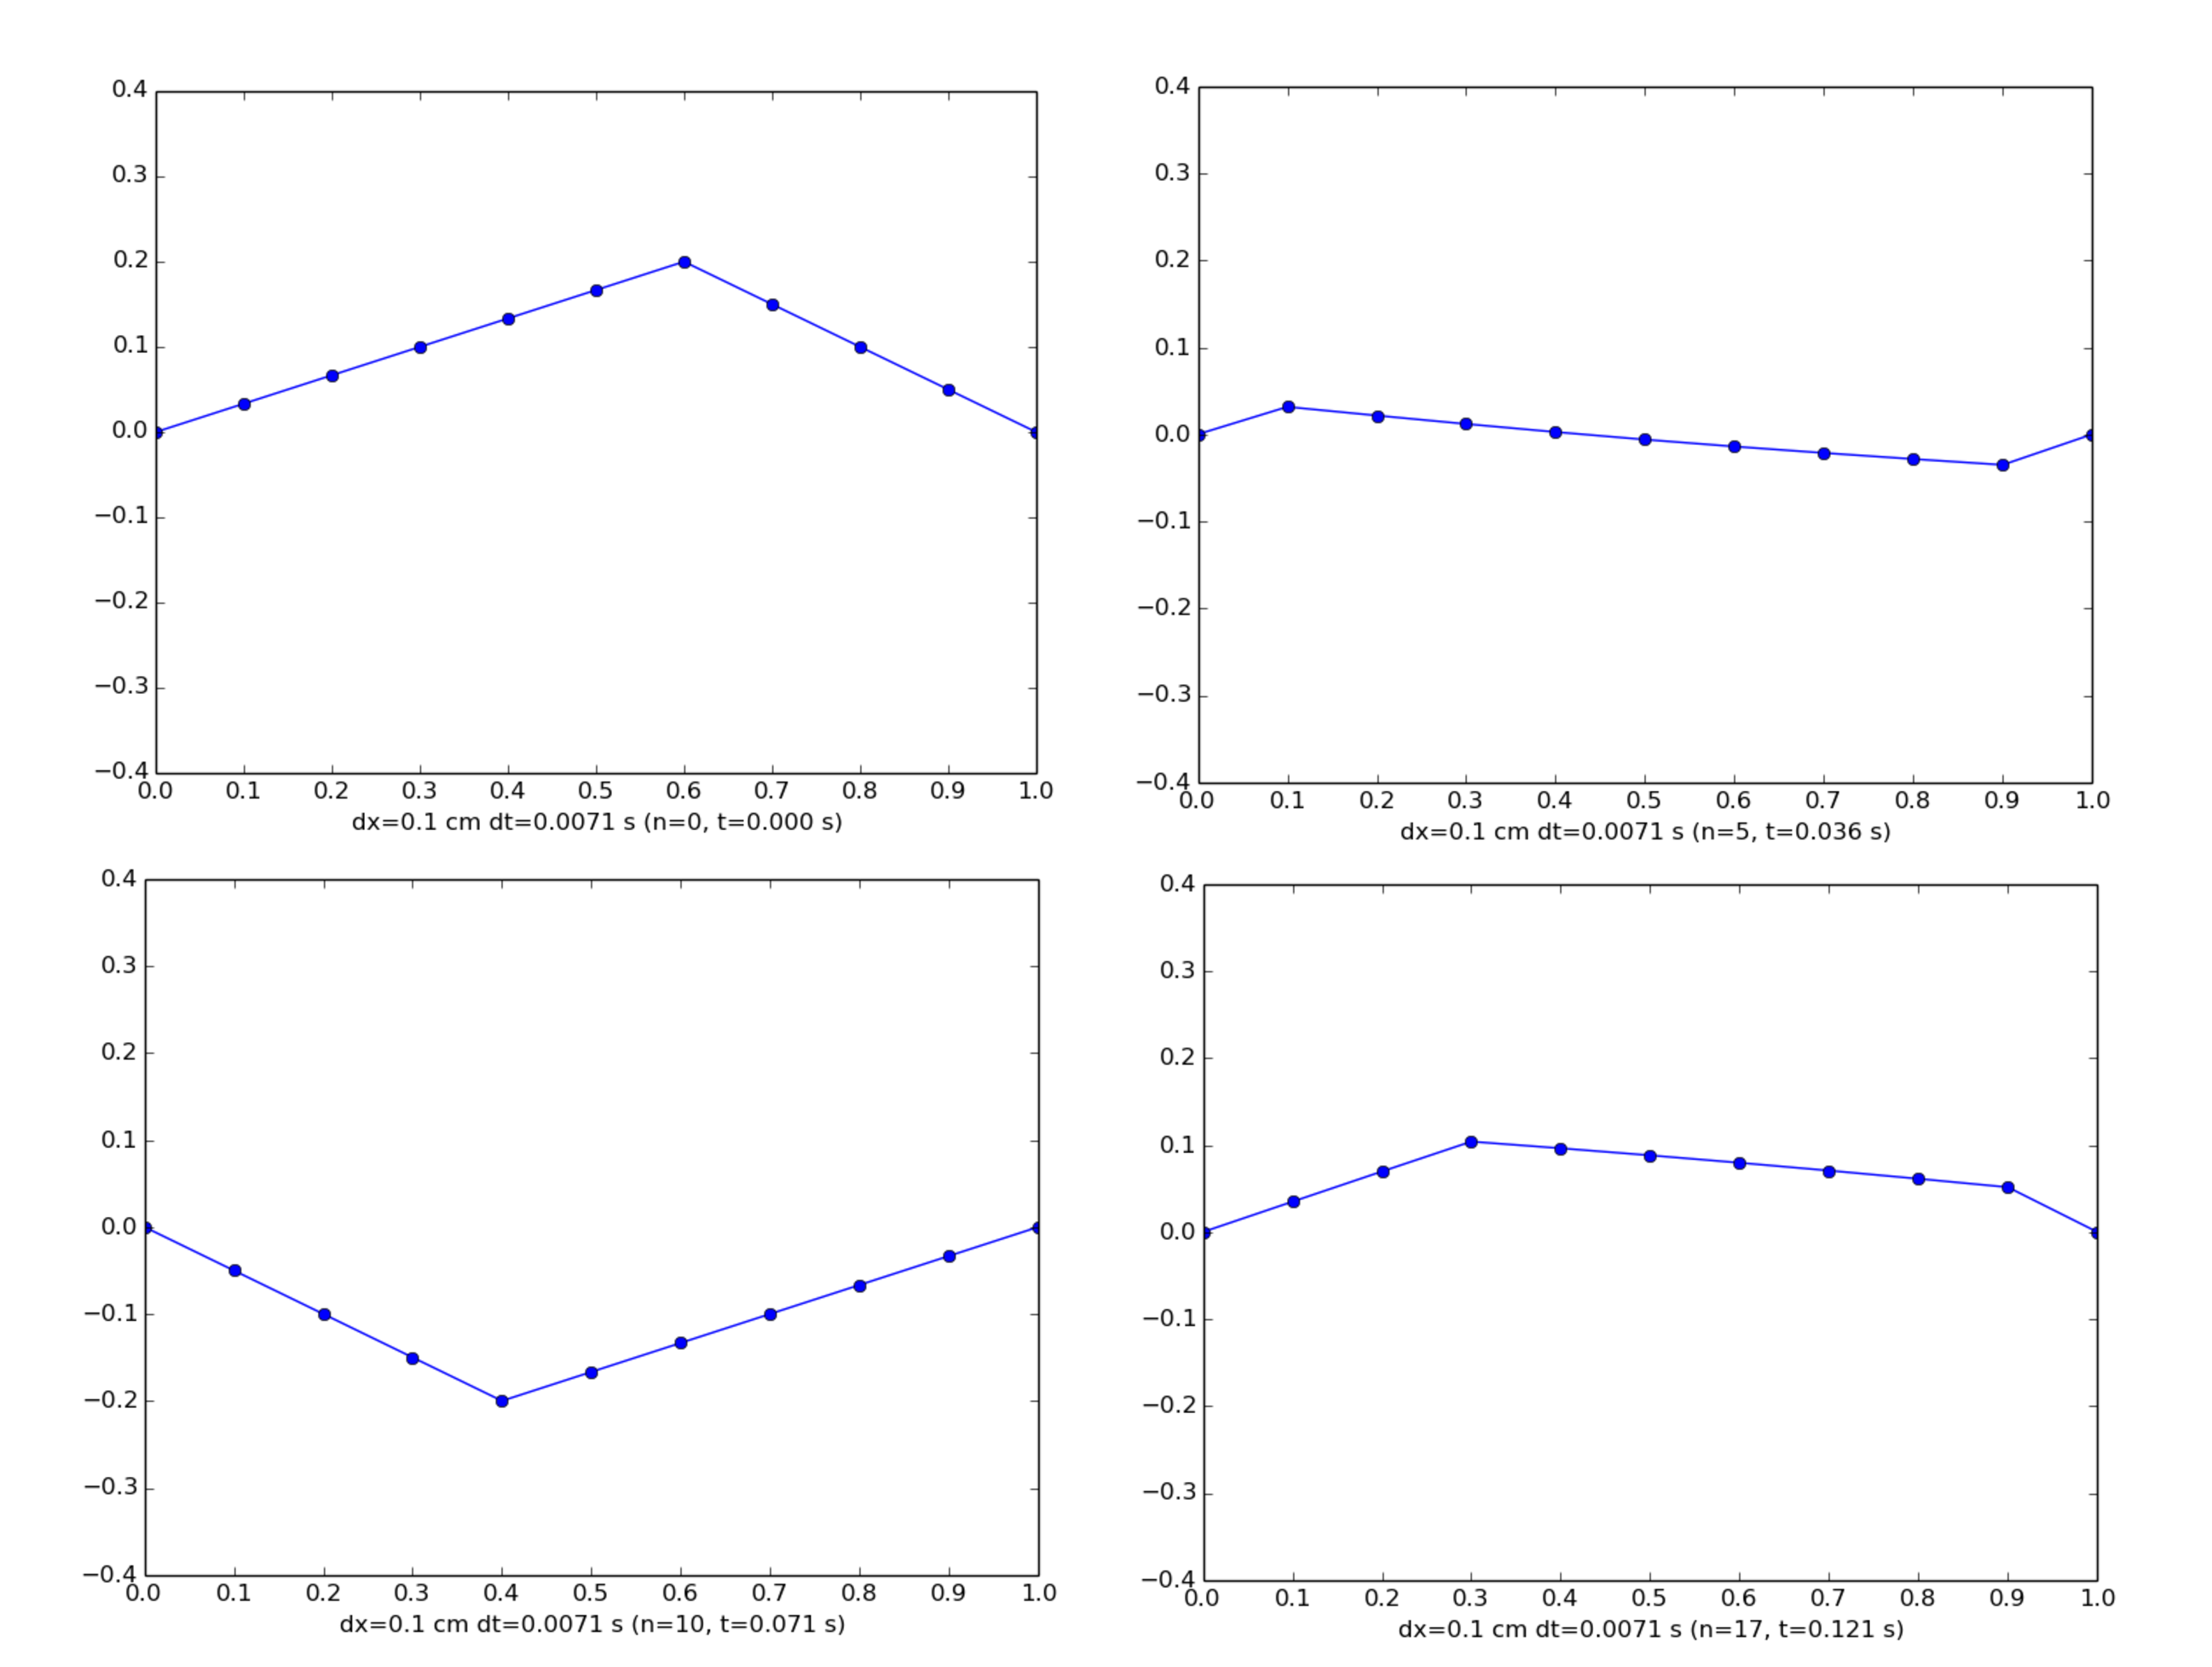
\includegraphics[width=1.0\linewidth]{graficas.pdf}
\caption{Vibración de la cuerda durante un ciclo de movimiento}
\label{fig:graficas}
\end{figure}

\subsection{Precisión del método}
Las Tablas \ref{tab:comparativa1}, \ref{tab:comparativa2} y \ref{tab:comparativa3} recogen
los resultados del cálculo de posición para diferentes intervalos $\Delta{x}$, mostrando
entre paréntesis el error $\epsilon = |y_i - y_{analitico}|$ por cada valor calculado.
Para ello se ha utilizado el resultado para el valor $(x,t)$ correspondiente proporcionado
por la solución analítica obtenida en la sección \ref{sec:sol_analitica}.

Como puede observarse, incluso con una división en intervalos de $\Delta{x} = 0.2$ cm, se 
obtiene una buena precisión comparada con la solución analítica, ya que únicamente existe
diferencia a partir de la cuarta cifra decimal. Esta diferencia se reduce, como puede
observarse en las Tablas \ref{tab:comparativa2} y \ref{tab:comparativa3}, al incrementar
el número de intervalos en los que se divide la cuerda, lo que reduce no solamente el
valor de $\Delta{x}$ sino también el de $\Delta{t}$ que se encuentra relacionado
directamente con este. Una reducción en el tamaño de un paso de tiempo significa que es
necesario llevar a cabo un mayor número de cálculos para alcanzar un determinado instante
de tiempo.

\begin{table}
\center
\begin{tabular}{ c c c c c }
\hline
Paso & 0.20 & 0.40 & 0.60 & 0.80 \\
\hline
\hline
0 & 0.0667 (0.0000) & 0.1333 (0.0000) & 0.2000 (0.0008) & 0.1000 (0.0000) \\
1 & 0.0644 (0.0002) & 0.1299 (0.0002) & 0.1132 (0.0002) & 0.0977 (0.0002) \\
2 & 0.0632 (0.0002) & 0.0443 (0.0004) & 0.0276 (0.0004) & 0.0132 (0.0002) \\
3 & -0.0201 (0.0002) & -0.0390 (0.0004) & -0.0557 (0.0004) & -0.0701 (0.0006) \\
4 & -0.1023 (0.0006) & -0.1201 (0.0002) & -0.1368 (0.0006) & -0.0690 (0.0002) \\
5 & -0.1000 (0.0000) & -0.2000 (0.0008) & -0.1333 (0.0000) & -0.0667 (0.0000) \\
% 6 & -0.0977 (0.0002) & -0.1132 (0.0002) & -0.1299 (0.0002) & -0.0644 (0.0002) \\
% 7 & -0.0132 (0.0002) & -0.0276 (0.0004) & -0.0443 (0.0004) & -0.0632 (0.0002) \\
% 8 & 0.0701 (0.0006) & 0.0557 (0.0004) & 0.0390 (0.0004) & 0.0201 (0.0002) \\
% 9 & 0.0690 (0.0002) & 0.1368 (0.0006) & 0.1201 (0.0002) & 0.1023 (0.0006) \\
% 10 & 0.0667 (0.0000) & 0.1333 (0.0000) & 0.2000 (0.0008) & 0.1000 (0.0000) \\
\end{tabular}
\caption{Precisión del método comparado con la solución analítica para $\Delta{x} = 0.2$ cm}
\label{tab:comparativa1}
\end{table}

\begin{table}
\center
\begin{tabular}{ c c c c c }
\hline
Paso & 0.10 & 0.20 & 0.30 & 0.40 \\
\hline
\hline
0 & 0.0333 (0.0000) & 0.0667 (0.0000) & 0.1000 (0.0000) & 0.1333 (0.0000) \\
1 & 0.0327 (0.0000) & 0.0655 (0.0000) & 0.0985 (0.0000) & 0.1316 (0.0000) \\
2 & 0.0322 (0.0000) & 0.0645 (0.0000) & 0.0971 (0.0000) & 0.1300 (0.0004) \\
3 & 0.0318 (0.0000) & 0.0638 (0.0000) & 0.0961 (0.0004) & 0.0871 (0.0001) \\
4 & 0.0316 (0.0000) & 0.0634 (0.0004) & 0.0538 (0.0001) & 0.0446 (0.0001) \\
5 & 0.0315 (0.0004) & 0.0216 (0.0000) & 0.0119 (0.0001) & 0.0026 (0.0001) \\
% 6 & -0.0100 (0.0000) & -0.0200 (0.0000) & -0.0296 (0.0001) & -0.0388 (0.0001) \\
% 7 & -0.0515 (0.0004) & -0.0612 (0.0000) & -0.0706 (0.0001) & -0.0796 (0.0001) \\
% 8 & -0.0511 (0.0000) & -0.1021 (0.0005) & -0.1112 (0.0000) & -0.1200 (0.0000) \\
% 9 & -0.0506 (0.0000) & -0.1011 (0.0000) & -0.1515 (0.0004) & -0.1600 (0.0000) \\
% 10 & -0.0500 (0.0000) & -0.1000 (0.0000) & -0.1500 (0.0000) & -0.2000 (0.0008) \\
\end{tabular}
\caption{Precisión del método comparado con la solución analítica para $\Delta{x} = 0.1$ cm}
\label{tab:comparativa2}
\end{table}

\begin{table}
\center
\begin{tabular}{ c c c c c }
\hline
Paso & 0.05 & 0.10 & 0.15 & 0.20 \\
\hline
\hline
0 & 0.0167 (0.0000) & 0.0333 (0.0000) & 0.0500 (0.0000) & 0.0667 (0.0000) \\
1 & 0.0165 (0.0000) & 0.0330 (0.0000) & 0.0495 (0.0000) & 0.0661 (0.0000) \\
2 & 0.0163 (0.0000) & 0.0327 (0.0000) & 0.0491 (0.0000) & 0.0655 (0.0000) \\
3 & 0.0162 (0.0000) & 0.0324 (0.0000) & 0.0487 (0.0000) & 0.0650 (0.0000) \\
4 & 0.0161 (0.0000) & 0.0322 (0.0000) & 0.0484 (0.0000) & 0.0646 (0.0000) \\
5 & 0.0160 (0.0000) & 0.0320 (0.0000) & 0.0481 (0.0000) & 0.0642 (0.0000) \\
% 6 & 0.0159 (0.0000) & 0.0319 (0.0000) & 0.0478 (0.0000) & 0.0638 (0.0000) \\
% 7 & 0.0159 (0.0000) & 0.0317 (0.0000) & 0.0476 (0.0000) & 0.0636 (0.0000) \\
% 8 & 0.0158 (0.0000) & 0.0316 (0.0000) & 0.0475 (0.0000) & 0.0634 (0.0004) \\
% 9 & 0.0158 (0.0000) & 0.0316 (0.0000) & 0.0474 (0.0004) & 0.0425 (0.0000) \\
% 10 & 0.0158 (0.0000) & 0.0316 (0.0004) & 0.0266 (0.0000) & 0.0216 (0.0000) \\
\end{tabular}
\caption{Precisión del método comparado con la solución analítica para $\Delta{x} = 0.05$ cm}
\label{tab:comparativa3}
\end{table}

\subsection{Caso con amortiguamiento}
En el caso de la cuerda con amortiguamiento es necesario utilizar las expresiones
completas dadas por las ecuaciones \eqref{eq:paso_inicial} y \eqref{eq:pasos_siguientes}
y que incluyen el parámetro $B = 2.0$.
Utilizando este esquema para la solución numérica se obtienen los resultados recogidos en
la Tabla \ref{tab:est_velocidad_amortiguado}.

En este caso, como era de esperar, la cuerda no puede recuperar su posición inicial ya que
pierde energía debido a la fuerza de amortiguamiento. Así, la altura de la cuerda es 
cada vez menor, hasta que para cierto instante de tiempo detiene prácticamente su
movimiento.

Utilizando la solución numérica puede estimarse el tiempo para el que el movimiento de la
cuerda se detiene dentro de un tolerancia determinada. Se ha determinado en qué momento
cada uno de los nodos de la cuerda se encuentran en el punto $0.0$ con un velocidad $0.0$
teniendo en cuenta una tolerancia de $0.0005$ en ambos casos. Se ha comprobado que esto
sucede para un número de pasos igual a 1300, por lo que se estima que la vibración de la
cuerda se detiene para $1300 * 0.0071 = 9.23$ segundos desde su puesta en marcha.

\begin{table}
\center
\begin{small}
\begin{tabular}{ c c c c c }
\hline
Paso & 0.30 & 0.40 & 0.50 & 0.60 \\
\hline
\hline
0 & 0.10 (-0.21) & 0.13 (-0.24) & 0.17 (-0.25) & 0.20 (-6.07) \\
1 & 0.10 (-0.19) & 0.13 (-0.22) & 0.16 (-6.02) & 0.16 (-5.97) \\
2 & 0.10 (-0.14) & 0.13 (-5.92) & 0.12 (-5.89) & 0.11 (-5.92) \\
3 & 0.10 (-5.79) & 0.09 (-5.78) & 0.08 (-5.83) & 0.07 (-5.78) \\
4 & 0.05 (-5.65) & 0.05 (-5.70) & 0.04 (-5.67) & 0.03 (-5.70) \\
5 & 0.01 (-5.60) & 0.01 (-5.55) & -0.00 (-5.58) & -0.01 (-5.55) \\
6 & -0.03 (-5.46) & -0.03 (-5.47) & -0.04 (-5.42) & -0.05 (-5.47) \\
7 & -0.06 (-5.41) & -0.07 (-5.34) & -0.08 (-5.37) & -0.09 (-5.34) \\
8 & -0.10 (-5.29) & -0.11 (-5.31) & -0.12 (-5.26) & -0.13 (0.20) \\
9 & -0.14 (0.19) & -0.15 (-5.21) & -0.16 (0.23) & -0.13 (0.22) \\
10 & -0.14 (0.19) & -0.19 (5.65) & -0.16 (0.23) & -0.12 (0.22) \\
11 & -0.14 (5.56) & -0.15 (5.55) & -0.15 (5.60) & -0.12 (0.20) \\
12 & -0.10 (5.45) & -0.11 (5.51) & -0.11 (5.48) & -0.12 (5.51) \\
13 & -0.06 (5.39) & -0.07 (5.38) & -0.07 (5.43) & -0.08 (5.38) \\
14 & -0.02 (5.26) & -0.03 (5.31) & -0.04 (5.28) & -0.04 (5.31) \\
15 & 0.02 (5.21) & 0.01 (5.16) & 0.00 (5.19) & -0.01 (5.16) \\
16 & 0.05 (5.09) & 0.05 (5.10) & 0.04 (5.05) & 0.03 (5.10) \\
17 & 0.09 (-0.13) & 0.08 (4.97) & 0.08 (5.00) & 0.07 (4.97) \\
18 & 0.09 (-0.16) & 0.12 (-0.19) & 0.11 (4.90) & 0.10 (4.94) \\
19 & 0.09 (-0.18) & 0.12 (-0.20) & 0.15 (-0.21) & 0.14 (4.86) \\
20 & 0.09 (-0.17) & 0.12 (-0.20) & 0.14 (-0.20) & 0.17 (-5.25) \\
% 21 & 0.09 (-0.16) & 0.11 (-0.18) & 0.14 (-5.21) & 0.14 (-5.16) \\
% 22 & 0.08 (-0.12) & 0.11 (-5.13) & 0.11 (-5.10) & 0.10 (-5.13) \\
% 23 & 0.08 (-5.02) & 0.08 (-5.01) & 0.07 (-5.05) & 0.06 (-5.01) \\
% 24 & 0.05 (-4.90) & 0.04 (-4.94) & 0.03 (-4.92) & 0.03 (-4.95) \\
\end{tabular}
\end{small}
\caption{Posición y velocidad de la cuerda amortiguada para $\Delta{x} = 0.1$ cm}
\label{tab:est_velocidad_amortiguado}
\end{table}

En la Figura \ref{fig:sol_amortiguada} se muestra el código utilizado en este caso para el
cálculo de la solución numérica, que es similar al mostrado en Figura \ref{fig:sol_basica}
pero donde se ha modificado el cálculo del paso inicial y siguientes. En este caso
únicamente se incluye el código correspondiente a los pasos iterativos, ya que el resto
es idéntico al mostrado en la Figura \ref{fig:sol_basica}. Los cambios en las expresiones
utilizadas se encuentran marcados en el código.

\section{Conclusiones}
Se ha llevado a cabo la resolución de la ecuación de la cuerda vibrante mediante la
aplicación de un método numérico consistente en la aproximación de las derivadas mediante
diferencias finitas. Se ha obtenido un esquema iterativo que ha sido implementado utilizando
el lenguaje de programación Python y que ha permitido obtener la posición y velocidad de
la cuerda para diferentes instantes de tiempo.

Por otro lado, la precisión del método numérico ha sido comparada con solución analítica,
que ha sido obtenida mediante la aplicación del método de separación de variables. Hay que
tener en cuenta que la solución analítica no es completamente exacta debido a que incluye
el cálculo de elementos de una serie de Fourier. Sin embargo, para la obtención de los
resultados analíticos se ha calculado un número alto de elementos de la serie con el fin
de conseguir una alta precisión en el resultado.

Durante la comparación de los resultados se ha observado que el método numérico obtiene
una buena precisión incluso para subdivisiones espaciales y temporales \emph{grandes}. Como
era de esperar, la precisión puede aumentarse incrementando el número de nodos y, en
consecuencia, reduciendo el tamaño del paso de tiempo. El aumento de la precisión repercute
directamente en el número de cálculos necesarios, debido tanto al incremento en el
número de nodos a calcular por paso como al aumento en el número de pasos necesarios para
alcanzar un determinado instante de tiempo.

El estudio de la cuerda vibrante se ha llevado a cabo en dos casos distintos: sin y con
amortiguación. En el caso sin amortiguación la progresión de la cuerda es periódica, y la
frecuencia de su oscilación ha podido determinarse con la búsqueda de un ciclo completo por
simple inspección de los resultados para cierto número de pasos de tiempo. Por otro lado,
en el caso de la cuerda amortiguada se ha comprobado que la amplitud de su movimiento
disminuye con el tiempo y que finalmente se detiene. Se ha estimado el intervalo necesario
para la detención de la cuerda buscando el primer paso de tiempo para el cual todos los
nodos se encuentran sobre el eje X y tienen una velocidad nula, teniendo en cuenta cierta
tolerancia para estos valores. 

Como conclusión final, en este caso el método numérico es mucho más fácil de desarrollar y
utilizar para obtener resultados que la solución numérica, que requiere la resolución de
las series de Fourier y su posterior cálculo para cierto número de coeficientes, teniendo
en cuenta, eso sí, los aspectos relacionados con la precisión del método numérico comentados
anteriormente.

\begin{figure}
\inputminted[linenos, lastline=54, fontsize=\footnotesize, tabsize=2]{python}
{../sol_analitica.py}
\caption{Código para el calculo de la solución analítica de la cuerda vibrante}
\label{fig:sol_analitica}
\end{figure}

\begin{figure}
\inputminted[linenos, lastline=56, fontsize=\footnotesize, tabsize=2]{python}
{../sol_sin_amortiguar.py}
\caption{Código para el cálculo de la solución numérica para el caso no amortiguado}
\label{fig:sol_basica}
\end{figure}

\begin{figure}
\inputminted[linenos, firstline=29, firstnumber=29, lastline=52, fontsize=\footnotesize, tabsize=2]{python}
{../sol_amortiguada.py}
\caption{Código para el cálculo de la solución numérica para el caso amortiguado}
\label{fig:sol_amortiguada}
\end{figure}

\nocite{*}

\bibliographystyle{plain}
\bibliography{biblio}

\end{document}